\documentclass[11pt,a4paper]{article}
\usepackage[spanish]{babel}			%Encabezados automaticos en español
\usepackage{listings}				%Utilizar codigo de un programa
\usepackage{url}					%Ingresar url
\usepackage{graphicx}				%Ingresar imagenes
\usepackage[usenames,dvipsnames]{color}					%Libreria para colores
\usepackage{amsmath,amsfonts,amsthm} % Math packages for equations
\usepackage[hang, small, labelfont=bf, up, textfont=it]{caption} % Custom captions under/above tables and figures
\usepackage{float}
\setlength{\parskip}{12pt}			%espacio entre parrafo
\setlength{\parindent}{0pt}			%espacio de sangria
\usepackage{enumerate}
\usepackage{subfigure}

\usepackage{pdfpages}
\usepackage[left=4cm,right=3cm,top=4cm,bottom=3cm]{geometry}

\author{Mario Gutiérrez \\ 1549273}
\title{Optimización de flujo en redes\\ 
\textbf{Portafolio}}

\begin{document}
\maketitle 

\setlength{\parindent}{0cm}

\section*{Descripción}

En el presente reporte se incluyen las distintas tareas realizadas a lo largo de la unidad de aprendizaje de optimización de flujo en redes (Enero-Junio 2019), además una breve descripción en base a la calificación obtenida.


\newpage

%---------------------------------------------------------
\section*{Tarea 1}

En esta práctica los principales errores fueron la falta de uso de ambiente matemático en las ecuaciones, el mal uso de números simples en párrafos, algunos errores de ortografía, la manera de referenciar las figuras, así como la bibliografía del documento.

\newpage
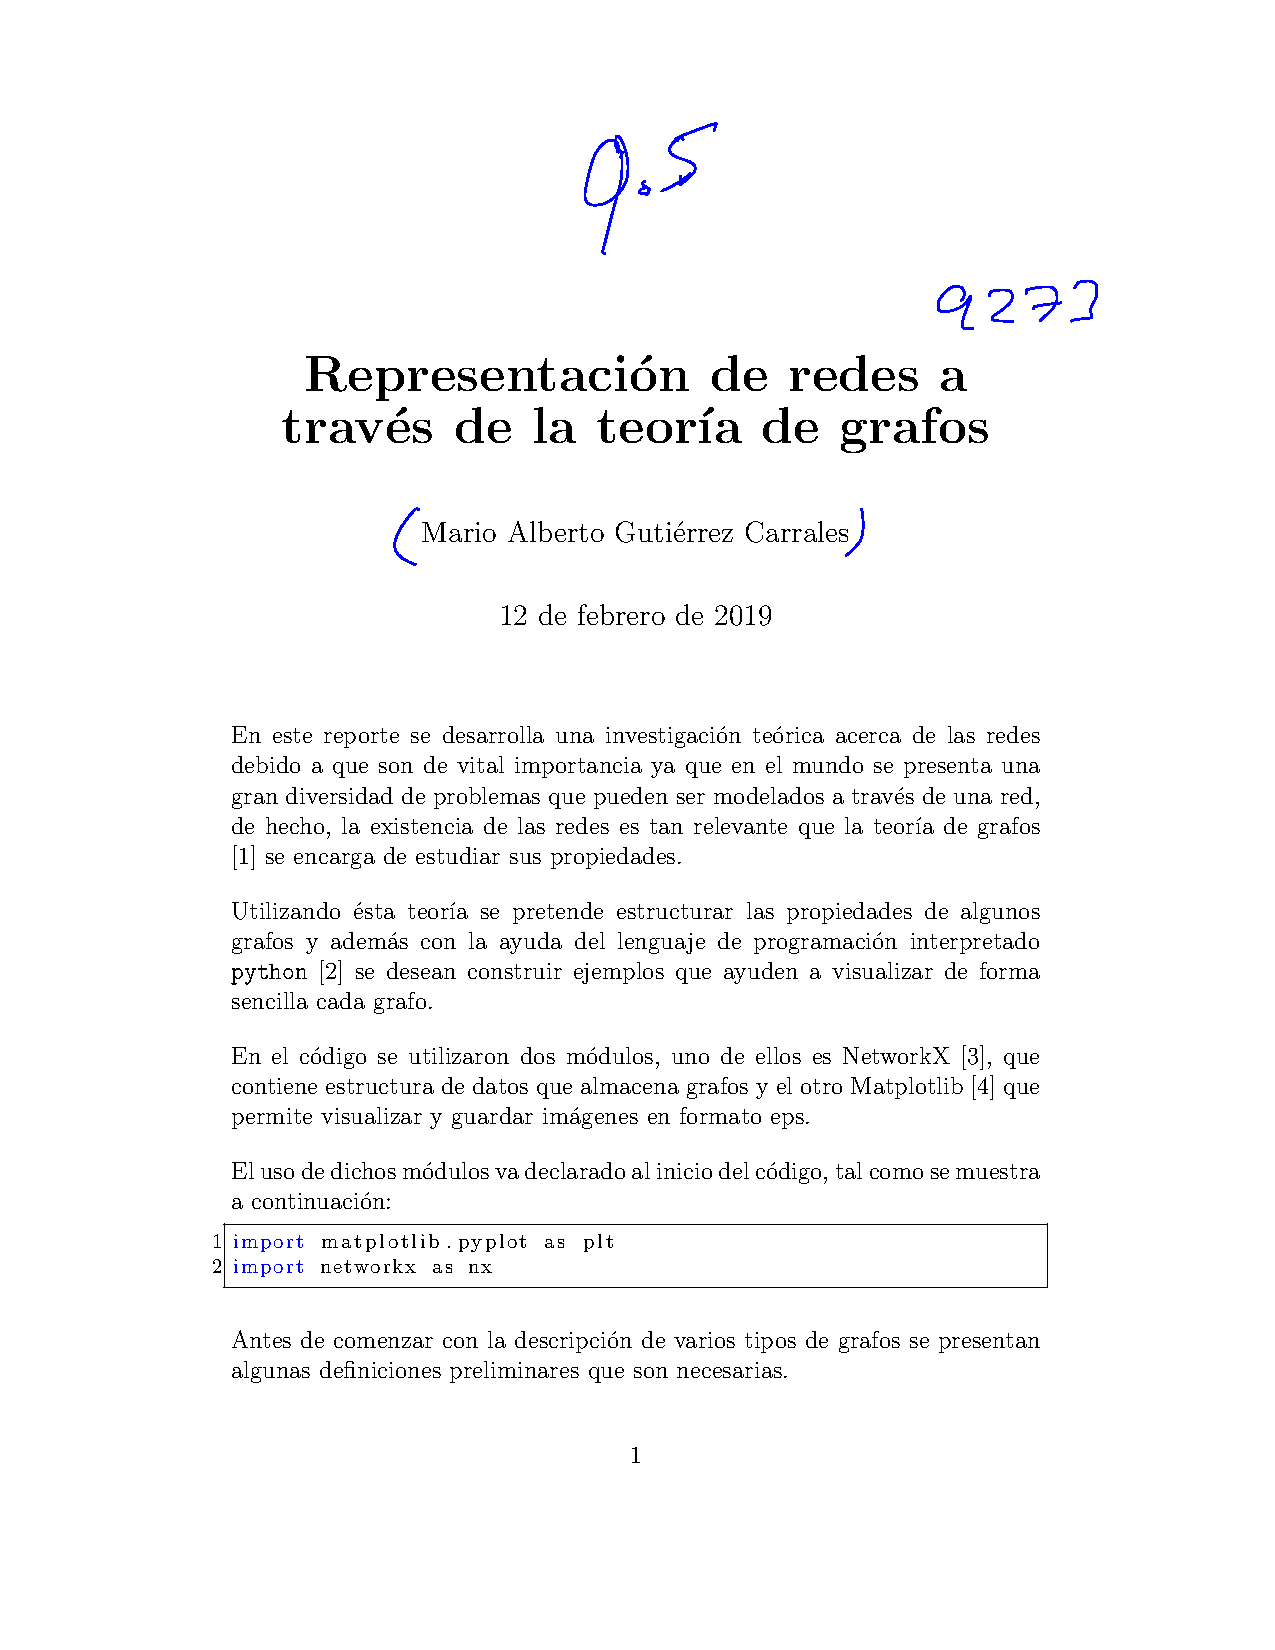
\includepdf[pages=-]{1.pdf}
%---------------------------------------------------------

%---------------------------------------------------------
\section*{Tarea 2}

En esta práctica los errores fueron breves y algunos de ellos fueron sobre identificar las palabras de otros idiomas y de ambiente computacional de otra tipografía, así como visualizar los nodos de los grafos de mayor tamaño.

\newpage
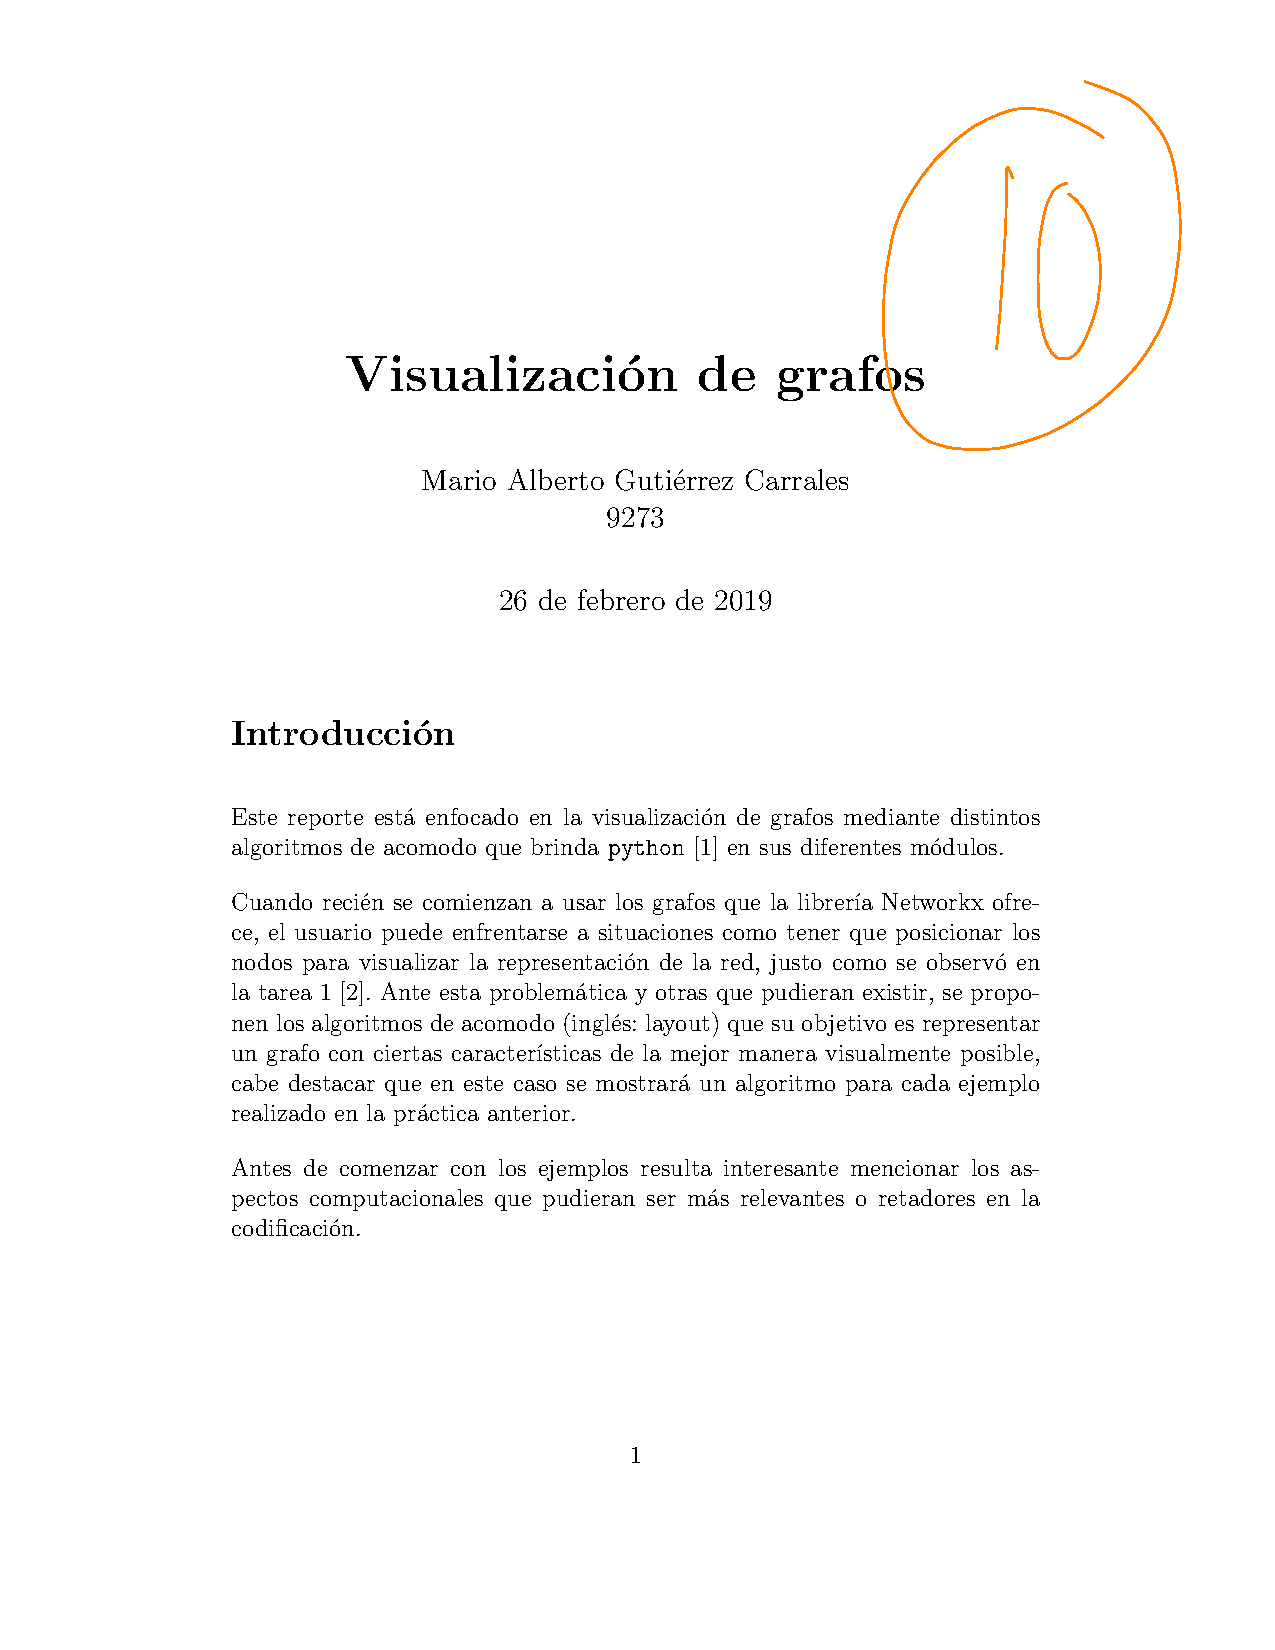
\includepdf[pages=-]{2.pdf}
%---------------------------------------------------------

%---------------------------------------------------------
\section*{Tarea 3}

En esta práctica hubo errores de ortografía, así como gráficos con falta de fundamento matemático para completar las conclusiones a lo que se pedía. 

\newpage
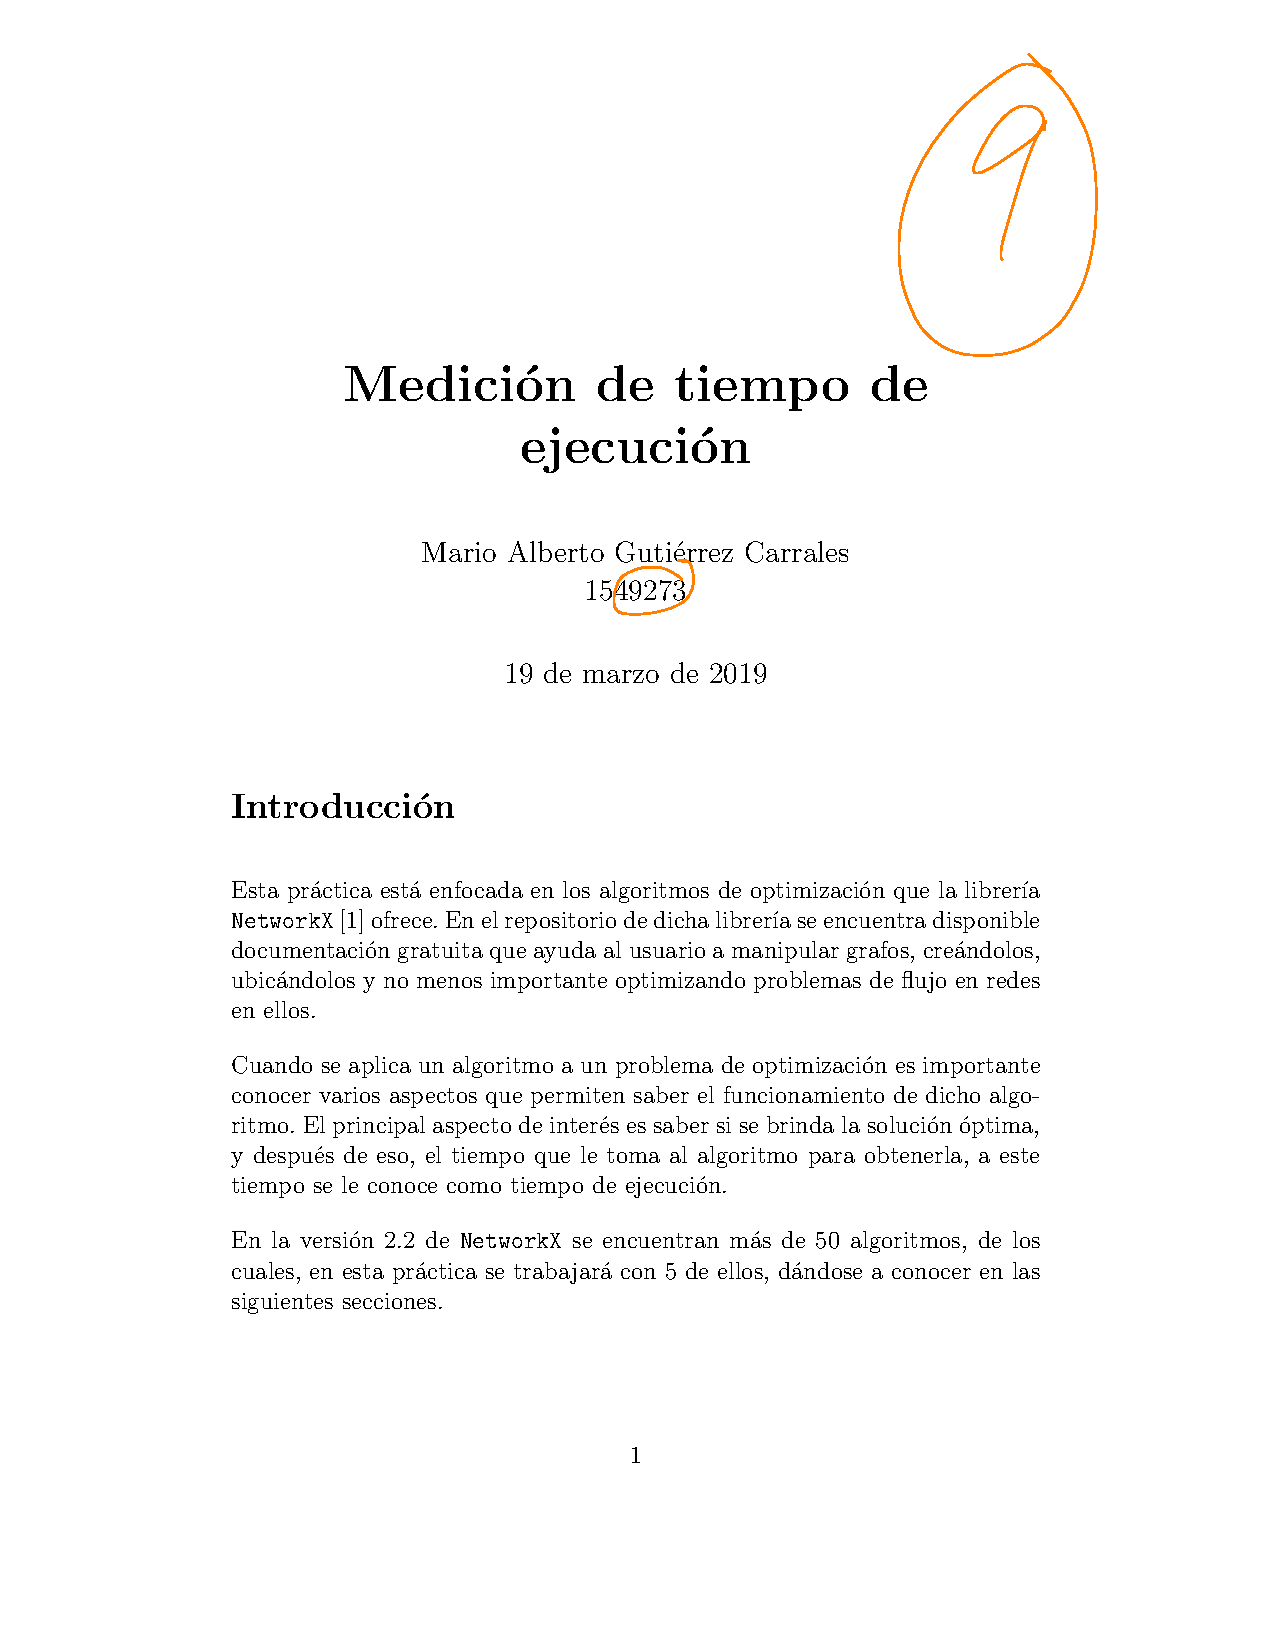
\includepdf[pages=-]{3.pdf}
%---------------------------------------------------------

%---------------------------------------------------------
\section*{Tarea 4}

En esta práctica los errores fueron en referirse a vértices y nodos de manera espontánea sin emplear un término fijo, así como arista y arco, también hubo algunos errores en el uso de ambiente matemático en las ecuaciones.

\newpage
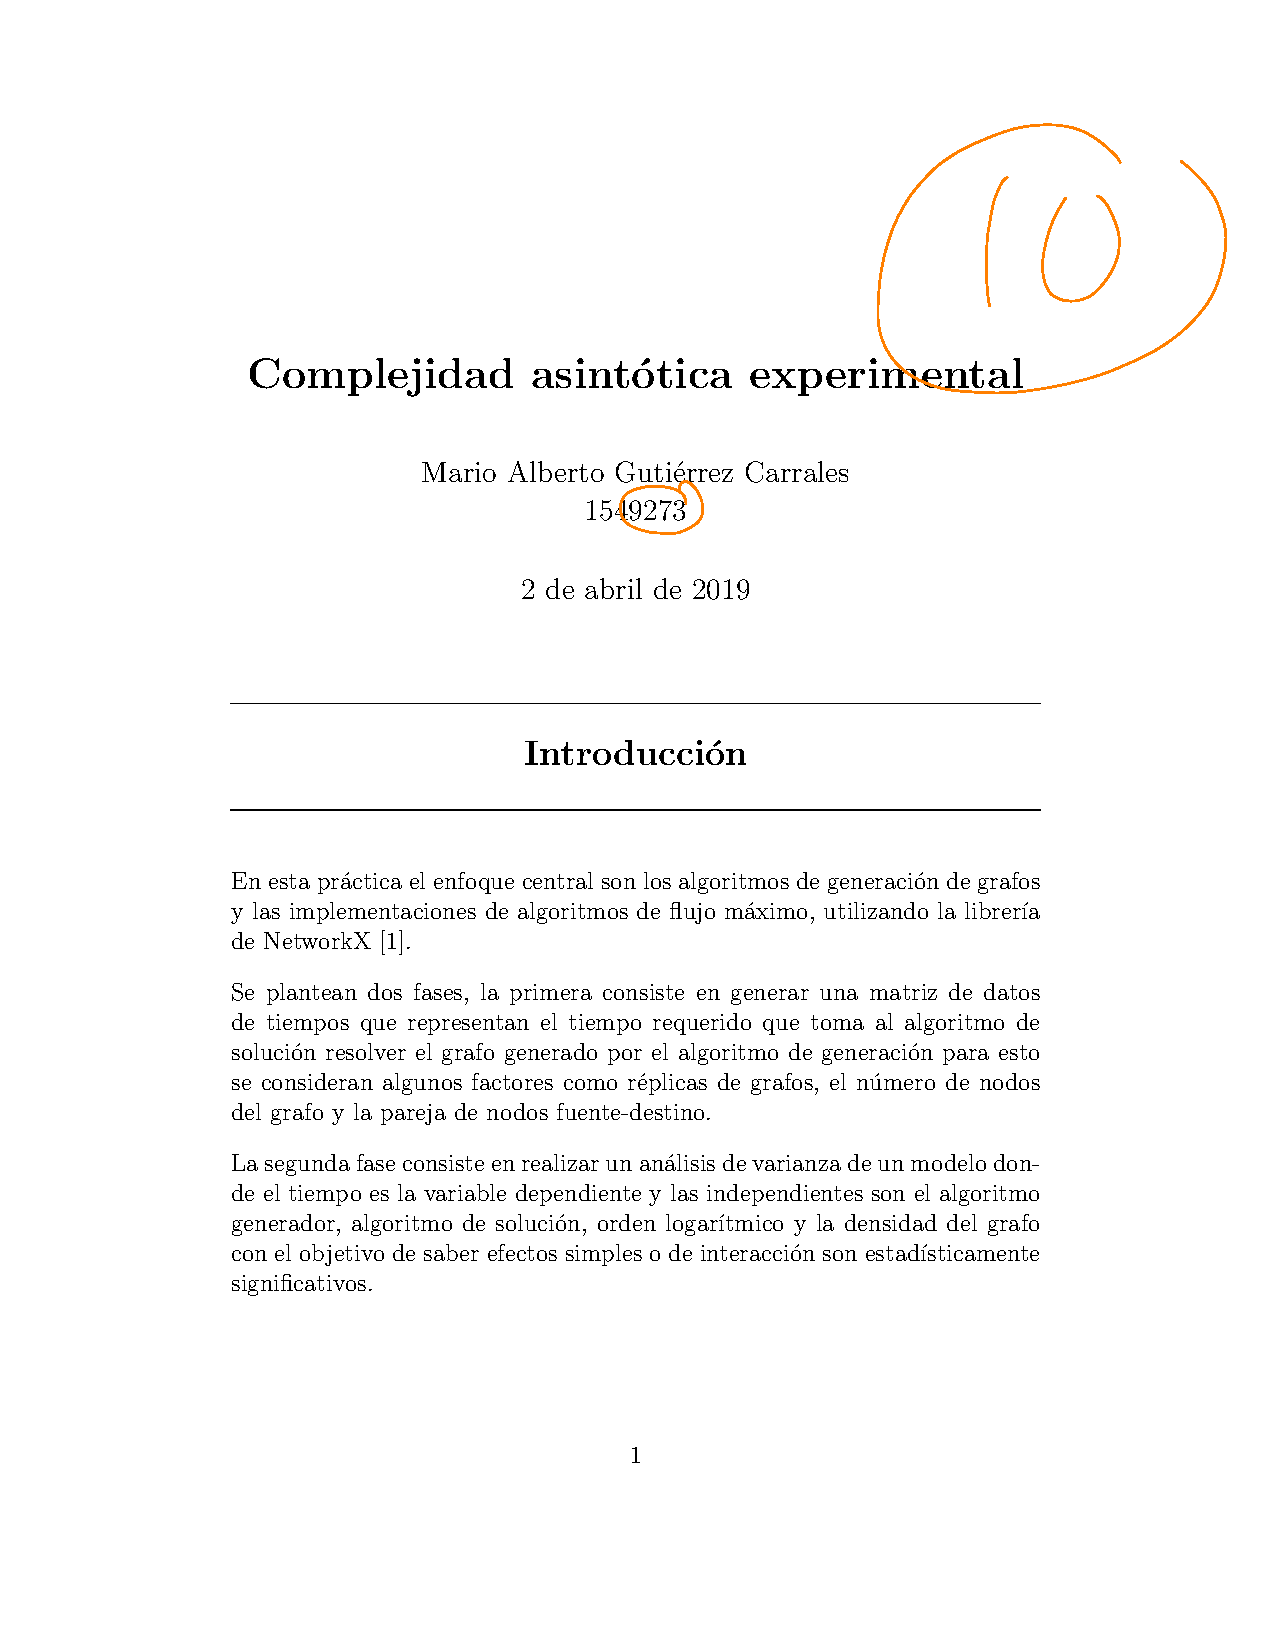
\includepdf[pages=-]{4.pdf}
%---------------------------------------------------------

%---------------------------------------------------------
\section*{Tarea 5}

En esta práctica los errores fueron correspondientes a la falta de uso de notas de pie de página para especificar detalle, algunos errores de ortografía, descripción de graficas en el \textit{caption} debajo de la figura.

\newpage
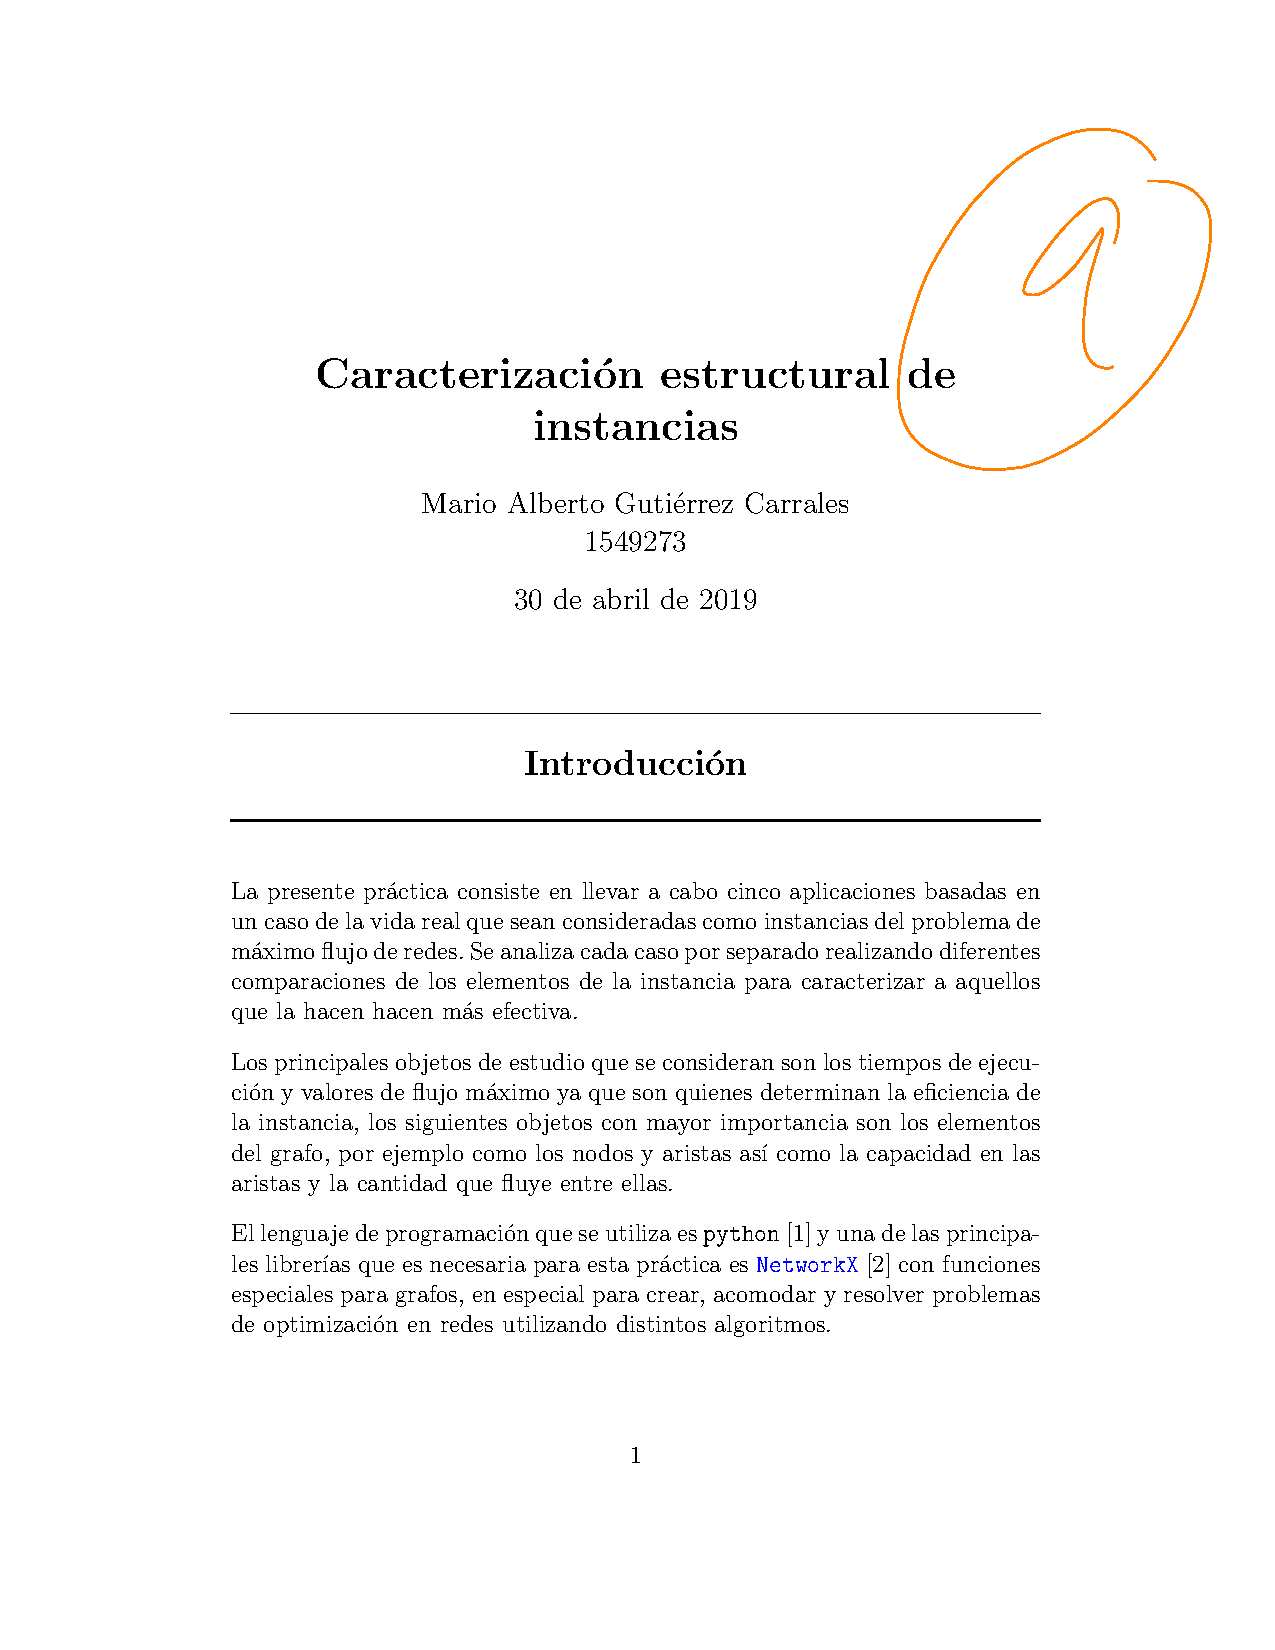
\includepdf[pages=-]{5.pdf}
%---------------------------------------------------------

%---------------------------------------------------------
\section*{Tarea 6}

Esta práctica no se había revisado, se adjunta para su revisión.

\newpage
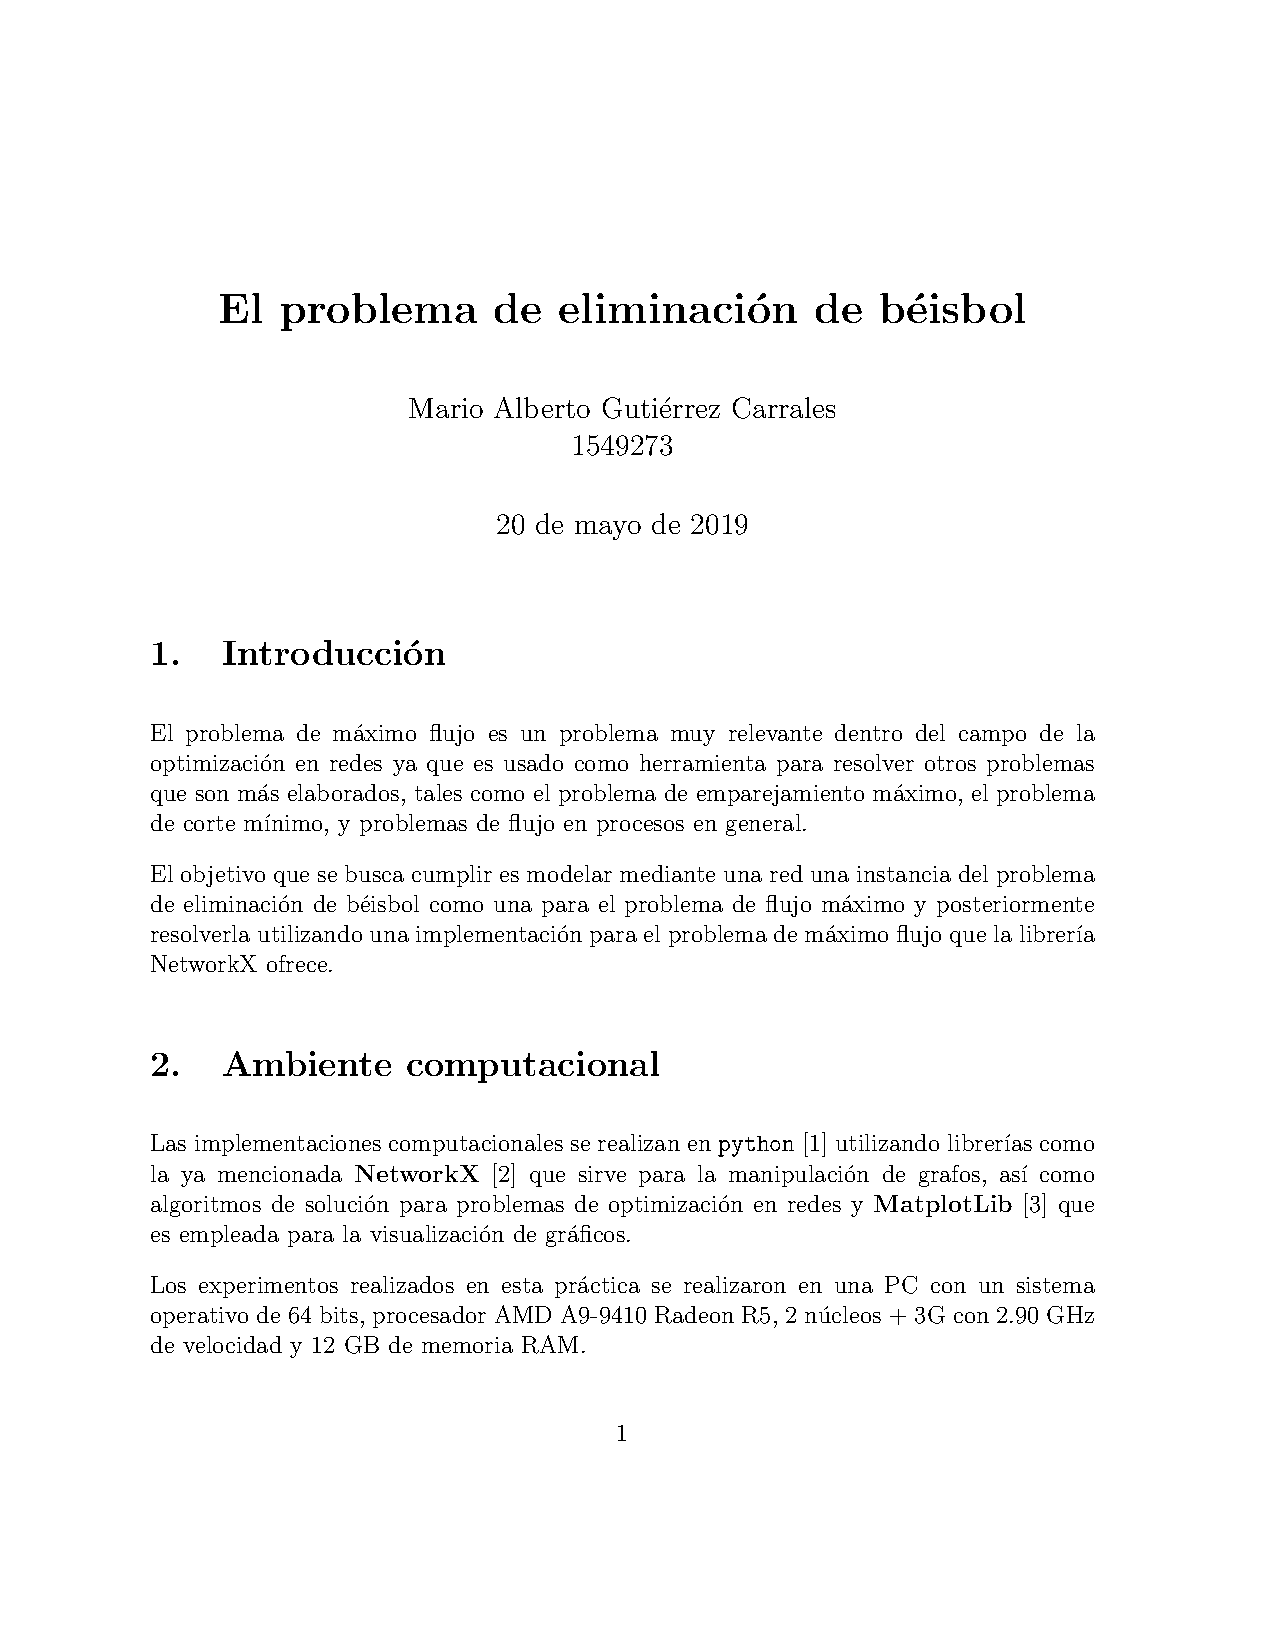
\includepdf[pages=-]{6.pdf}
%---------------------------------------------------------
\end{document}